%### 
\subsection{Fitness Functions}
%### 
\label{sec:fit}
One requirement of this work was to provide \xmlmate with the concept of pluggable fitness functions and 
give several examples that demonstrate the versatility of the approach. Luckily, \evosuite already provides 
a \texttt{FitnessFunction<T extends Chromosome>} generic interface, which can be employed on multiple 
levels of abstraction. To provide the pluggability on the level of  entire test suites there are implementers of
\texttt{FitnessFunction<XMLTestSuiteChromosome>}, and on the level of single test inputs -- ones of 
\texttt{FitnessFunction<XMLTestChromosome>}. 
Secondary evolution objectives have a very similar type topography; secondary objectives are sometimes useful 
as ``tie breakers'' when a decision between two chromosomes has to be made when both have equal fitness values,
but possess subtle differences that e.g.\ might lead to slightly more or less favorable crossover behavior in 
the future. The next sections describe some of the new fitness function implementations available with the 
extended and improved \xmlmate.
%### 
\subsubsection{Schema Coverage Fitness Function}
%###
\label{sec:fit:schema}
The very first extension from pure \java branch coverage and exception oriented fitness functions employed 
previously in \xmlmate is the \texttt{Schema Coverage} fitness function. Its goal is to maximize the number 
of schema rules used in the generated inputs. The reasoning behind this is that inputs which exhibit most of 
the features described in the specification should also trigger more functionality in the program under test. 
More concretely the schema coverage fitness value is computed as the average of the following three values:
\begin{description}
  \item[element coverage] describes how many element declarations were instantiated in the generated inputs, 
  including substitution group members. A substitution group consists of jointly declared elements, which 
  can take each other's place in the \xml. Additionally, the element coverage can reflect how many branches 
  of \texttt{choice} particles as well as how many of the optional elements are present in the produced files.
  This is somewhat reminiscent of the branch coverage criterion applied on the level of the input format
  definition instead of the executed code.
  \item[attribute coverage] is, similarly, a measure of how many attribute declarations were utilized, so its 
  value depends on both the optionality of the declarations and the number of generated elements (or more 
  precisely the number of elements carrying the corresponding attribute declarations).
  \item[transition coverage] roughly describes how many values of elements and attributes were explored. One of
  the most implementation-wise challenging features of the \xsd{} Language is the \texttt{pattern}
  facet that describes valid values of an element or attribute by means of a regular expression. These
  expressions have a different grammar than that of \java, \python or Perl regular expression
  languages, which, as an aside, presented another whole technical challenge.
  In order to be able to provide values conforming to those regular expressions an automaton based representation 
  has been put in place for the types of the elements and attributes by using the automaton
  library\cite{automaton} for \java.
  In fact, it worked so well, that there was longer any need in representing any type in a way other than by
  means of a deterministic finite automaton. This means that all types, including \texttt{string},
  \texttt{int}, \texttt{short}, \texttt{hexBinary}, have a corresponding automaton, which is cached in memory
  for performance reasons. Furthermore, with this representation it is very easy to apply additional facets
  like restrictions on length or number of fractional digits just by performing automaton based operations
  like union and intersection.
  Coming back to the topic of schema coverage, the transitions in these automata are the subject of its 
  transition coverage component which describes how many of the transitions of all the automata are being 
  used in the generated \xml files. This measure is indicative of the overall proportion of covered value space 
  over all type definitions regarded together.
\end{description}

If the element, attribute, and transition coverages are designated as $c_e$, $c_a$, and $c_t$ respectively and
are numbers between zero and one, the overall schema coverage fitness value can be computed as $1 -
\frac{c_e+c_a+c_t}{3}$, which makes this a \emph{minimization} fitness function, meaning that the genetic
algorithm of \evosuite will try to get the value as close to zero as possible, which is its default behavior.

In contrast with the initial intuition, the results of previous experiments did not 
show a strong correlation between high schema coverage and certain kinds of code coverage like 
branch or basic block coverage. This can be explained by the fact that it is not the abundance of different 
input values, but rather the specific values themselves, that are responsible for penetrating deeper into a 
program's logic and thus increasing the code coverage. This is why there is no separate evaluation of this
fitness function alone.

However, the schema coverage is a useful evolution guide for the purpose of creating a diverse starting
population which can then be further evolved with different purposes -- be it code coverage of particular program regions, or
other kinds of fitness criteria like closeness to integer overflows and the like.

Furthermore, there is no need in powering up any of the infrastructure involved with the usual ways of
measuring fitness -- no system under test, no brokers or converters are needed to compute the schema coverage
fitness. There is also no need for \texttt{IO} operations, as all \xml tree evaluations are processed
in-memory. This makes the Schema Coverage fitness function very efficient.

%### 
\subsubsection{Basic Block Coverage Fitness Function}
%###
A more or less direct transfer of \evosuite's \texttt{Instruction Count} fitness function is the 
\texttt{Basic Block Coverage} fitness function, which aims to maximize the number of basic blocks 
executed in the program under test. This fitness function makes heavy use of the Intel \pin
instrumentation framework -- in particular its definition of a basic block: a single entrance, 
single exit sequence of instructions in the program under test. However, because \pin is discovering the 
program dynamically as it is executed, its view of basic blocks can be somewhat unconventional. As an 
example consider the code on the left in \cref{lst:bblcode}, which, when compiled for the IA-32 
architecture, will yield instructions approximate to the ones on the 
right\footnote{From \url{https://software.intel.com/sites/landingpage/pintool/docs/67254/Pin/html/\#GRAN}}.
Classically speaking, each \mintinline{nasm}{addl} instruction is its own basic block; however, over the course
of program execution, when the different switch cases are entered, \pin will generate basic blocks, which
contain four instructions as the \texttt{.L7} case is entered, three basic blocks as the \texttt{.L6}
case is entered, and so forth. Furthermore, \pin breaks basic blocks on some other instructions like 
\texttt{cpuid}, \texttt{popf}, and \texttt{REP} prefixed instructions. This leads to a slight divergence 
from the expected values, but for the purposes of representing code coverage this has no negative 
consequences. As a matter of fact, this phenomenon is actually somewhat reminiscent of the LCSAJ
metric\cite{Hennell:1976:PA}, which only increases its worth as a fitness score component.
\begin{listing}[h]
\centering
\begin{minipage}[b]{0.49\textwidth}
	\centering
	\begin{ccode*}{linenos=false,frame=bottomline}
	switch(i) {
        case 4: total++;
        case 3: total++;
        case 2: total++;
        case 1: total++;
        case 0:
        default: break;
    	}
\end{ccode*}
	Example C Code
 \end{minipage}
%
 \begin{minipage}[b]{0.49\textwidth}
  \centering
  \begin{minted}[frame=bottomline]{nasm}
.L7:
        addl    $1, -4(%ebp)
.L6:
        addl    $1, -4(%ebp)
.L5:
        addl    $1, -4(%ebp)
.L4:
        addl    $1, -4(%ebp)
\end{minted}
  IA-32 Instructions
 \end{minipage}
 \caption{Example for Basic Block Idiosyncrasies in \pin}
 \label{lst:bblcode}
\end{listing}

The \texttt{Basic Block Coverage} fitness function is the first, but not the only to use the new binary 
backend feature set. Therefore it profits from an abstract fitness function prototype designed specifically 
to work with binary test subjects, which abstracts away and manages the responsibilities of communicating 
with the backend system, be it potential format converters, or the targeted program controlled by test 
drivers and monitored by pintools.
Like all subclasses of this \texttt{BinaryBackendFitnessFunction}, the \texttt{Basic Block Coverage} 
fitness function consists of two components: a \java class and a pintool written in \cpp.

The pintool's task is to instrument the targeted binary in such a way, that whenever it executes a 
basic block, which belongs to the binary image of interest (e.g.\ \texttt{libpng} -- a parameter given at the
start), its address is recorded in a set data structure. When the test driver, which is responsible for running 
the program under test, signals the completion of the processing of the currently evaluated inputs, 
the pintool sends the set as a packet to the \java class in \xmlmate.

It is the purpose of the fitness function's \java class to interpret the data received from the pintool.
In the case of the \texttt{Basic Block Coverage} fitness function, the data received represents the
set of starting addresses of the basic blocks that were found to be executed in the program under test. 
For each \xml in a test suite an individual set must be maintained in order to be able to profit 
from result caching: when a test suite is modified during the evolution step, not necessarily all
of its tests must have been changed and thus not all tests must be passed to a test driver for reevaluation, 
their previous result can be reused because it is still up-to-date. Virtue of the fact that the pintool 
builds a set out of the addresses of the executed blocks on its side already, the result for a single 
\xml can be stored as an array (\texttt{long[]}) without having to wrap a \texttt{Set} container around it.

However, when it comes to calculating the number of unique basic blocks covered by an 
entire test suite, each time a new set consisting of the union of the individual arrays belonging to all \xml
files in the suite must be created. At this point the very efficient \texttt{TLongHashSet} implementation from
the \emph{GNU Trove} collections mentioned in \cref{sec:trove} is very useful -- especially so because it
stores the \java primitive values directly instead of \emph{boxing} them in wrapper objects like the standard
\java collections do. Because Trove saves space and is faster, it is used in all following fitness functions
as a standard container provider.

The actual fitness value of a test suite according to the \texttt{Basic Block Coverage} fitness function 
is the number of unique basic blocks executed by all \xml files in the suite. Due to the dynamic nature 
of instrumentation with \pin it is impossible to know the total number of basic blocks in the program 
under test. One consequence of this is that this fitness function must be a maximization function -- meaning
that higher fitness values are considered better, which is somewhat atypical for \evosuite. Even though it has
some degree of support for maximization functions, multiple code defects surfaced during the development that
mostly had to do with hard-coded assumptions about the fitness function always being a minimization function.
These discovered defects were fixed.

%### 
\subsubsection{Basic Block Succession Fitness Function}
%### 
The \texttt{Basic Block Succession} fitness function is a continuation and an extension of the
\texttt{Basic Block Coverage} fitness function in that it is also heavily based on observing the execution of
basic blocks. However, this extension also considers the order in which the blocks are executed. More
specifically, for each basic block this fitness function aims to maximize the number of unique basic blocks
that are executed immediately after.
Put differently, the \texttt{Basic Block Succession} fitness function provides guidance for maximizing the
number of control paths of length two taken by the program under test. This makes it, strictly speaking, a
specialization of the more general \emph{path coverage} criterion, which indicates whether every possible route
of control in the targeted program has been executed.
According to the
author\footnote{http://lcamtuf.blogspot.de/2014/08/a-bit-more-about-american-fuzzy-lop.html} of the
\texttt{American Fuzzy Lop} smart fuzzing tool\cite{afl}, this specialized strategy strikes a good balance
between fitness function complexity and effectiveness, and is very helpful in finding defects.

To accomplish its task, the pintool maintains a map, which contains an address for each basic block that was
observed to be executed as a key. Each key is assigned as value a set of all basic blocks that were executed
immediately after it -- be it by fall-through, call, return, or conditional jump. 

The \java part of the \texttt{Basic Block Succession} fitness function receives this map data for each file in
the suite, and collates and merges it into a single basic block successor graph in order to determine the
fitness of the entire suite. The fitness value is then calculated as the number of edges in this graph. 
\Cref{fig:bblsuc} gives a small example for this process. The vertices represent basic blocks and the edges
indicate succession of control between them. Subfigures (a) and (b) represent succession maps corresponding to
two input files -- each of them has a score of 3 because each has 3 edges. The merged graph has a score of 5 as
it contains 5 unique successions.

\begin{figure}[h]
	\centering
	\begin{subfigure}[b]{0.3\textwidth}
	\begin{tikzpicture}[->,>=stealth',shorten >=1pt,auto,node distance=2cm,thin,
	bbl/.style={rectangle, draw, font=\sffamily\small}]
		\node[bbl] (1) {1};
		\node[bbl] (2) [right of=1] {2};
		\node[bbl] (4) [below of=2] {4};
		\node[bbl] (3) [right = 1.5cm of {$(2)!0.5!(4)$}] {3};
		
		\path[every node/.style={font=\sffamily\small}]
		(1) edge [right]node {} (2)
			edge [right]node {} (4)
		(2) edge [right]node {} (3);
	\end{tikzpicture}
	\caption{First Graph}
	\end{subfigure} %
	~
	\begin{subfigure}[b]{0.3\textwidth}
	\begin{tikzpicture}[->,>=stealth',shorten >=1pt,auto,node distance=2cm, thin,
	bbl/.style={rectangle, draw, font=\sffamily\small}]
		\node[bbl] (1) {1};
		\node[bbl] (2) [right of=1] {2};
		\node[bbl] (4) [below of=2] {4};
		\node[bbl] (3) [right = 1.5cm of {$(2)!0.5!(4)$}] {3};
		
		\path[every node/.style={font=\sffamily\small}]
		(1) edge [right]node {} (2)
		(2) edge [right]node {} (4)
		(4) edge [right]node {} (3);
	\end{tikzpicture}
	\caption{Second Graph}
	\end{subfigure}%
	~
	\begin{subfigure}[b]{0.3\textwidth}
	\begin{tikzpicture}[->,>=stealth',shorten >=1pt,auto,node distance=2cm, thin,
	bbl/.style={rectangle, draw, font=\sffamily\small}]	
		\node[bbl] (1) {1};
		\node[bbl] (2) [right of=1] {2};
		\node[bbl] (4) [below of=2] {4};
		\node[bbl] (3) [right = 1.5cm of {$(2)!0.5!(4)$}] {3};
		
		\path[every node/.style={font=\sffamily\small}]
		(1) edge [right]node {} (2)
			edge [right]node {} (4)
		(2) edge [right]node {} (3)
			edge [right]node {} (4)
		(4) edge [right]node {} (3);
	\end{tikzpicture}
	\caption{Merged Graph}
	\end{subfigure}
    \caption{Example Block Succession}
  \label{fig:bblsuc}

\end{figure}

%### 
\subsubsection{Memory Access Fitness Function}
%###
\label{sec:memcov}
All previously described fitness functions are aimed at increasing a coverage of one sort or another; however,
in the context of using \xmlmate to try and find vulnerabilities in the system under test, this is not
necessarily the most appropriate approach. In order to be able to find vulnerabilities that have to do with
operations such as reading from and writing to memory, such as null pointer dereferences or buffer underflows
or overflows, the first na\"\i{}ve approach is to aim for a maximal number of memory reads and writes at a
maximal number of addresses. This is the idea behind the \texttt{Memory Access} fitness function, which, like
its cousin \texttt{Basic Block Coverage} fitness function, is a maximization function, with which it also shares
the \texttt{BinaryBackendFitnessFunction} as an ancestor. As before, this fitness function consists of a
pintool and its complementary \java class. 

The pintool stores memory addresses that were accessed by the program under test in a set, which it sends to
the \java class upon test completion.
The \java class is very similar to that of its cousin fitness function, in fact they share almost the entirety
of their code.

%###
\paragraph{Singleton Population} ~\\
%###
However, upon consideration of the current use case, the distinction between test suites and tests as
prescribed by \evosuite no longer seems appropriate -- instead it is preferable to evolve a population
of single \xml files in order to find one individual file that triggers faulty behavior. To satisfy this newly
appeared need, the concept of a \emph{singleton population} was introduced.

Using a singleton population is a compromise between \evosuite's need for the presence of test suites to
evolve, and the new need for only one set of files to be evolved. When the singleton population is used,
the population size of the genetic algorithm is limited to only one suite and the genetic algorithm itself is
modified accordingly -- among other adjustments by disabling elitism on the test suite level. Elitism is a
mechanism which ensures that the best individual (the best test suite in \evosuite's case) survives into the
next generation unaltered, so that fitness may never decrease from one generation to the next. 
When the singleton population is used, instead of engaging elitism on the level of entire test suites, there
is elitism among all the single files in the one suite being evolved, such that the one best file is
guaranteed survival. Note, that using elitism does not prevent the best individual from reproducing as its
copies may do so freely, and usually this is what leads to an improvement in fitness.
 
With the singleton population in place, there is only one test suite to evolve, consequently, the fitness
must now be calculated differently. The fitness of this single suite can no longer reflect the cumulative
result over all the tests, but must rather correspond to the fittest one of them. At the end of the
evolution this value will be considered the result of the search, or the pinnacle of evolution, if you will.

This routine can be improved by adding a secondary evolution objective, which considers a
mutation of the test suite as an improvement even if it has the same number of memory accesses in the best
test, yet cumulatively its tests cause more unique memory addresses to be accessed. 

There were considerations to model the use case of evolving a
set of files as a population of singleton test suites each containing a single file instead of the currently
employed population consisting of one suite. This, however, would have been unfavorable to the parallelization
efforts as per \cref{sec:par} because \evosuite does not allow parallel evaluation of test suites without a
major intrusion in its code base.
%### 
\subsubsection{Division by Zero Fitness Function}
%###
Like the \texttt{Memory Access} fitness function, the \texttt{Division by Zero} fitness function is also
designed to find vulnerabilities in the program under test instead of simply improving test input quality. In
particular, this fitness function aims to uncover a single class of denial of service vulnerabilities -
unhandled arithmetic exceptions that arise from performing division by zero.

When the program under test processes an input file, it usually executes multiple distinct division
instructions, and many of them multiple times, so there is no simple and obvious way to directly assign a
fitness value to an input file. The first idea is to record all observed instances of division and choose the
smallest absolute value of a divisor as the fitness score. \Cref{fig:div0} shows an example calculation of the
fitness score for a test suite that consists of two input files. 

\begin{figure}[htb]
\centering
  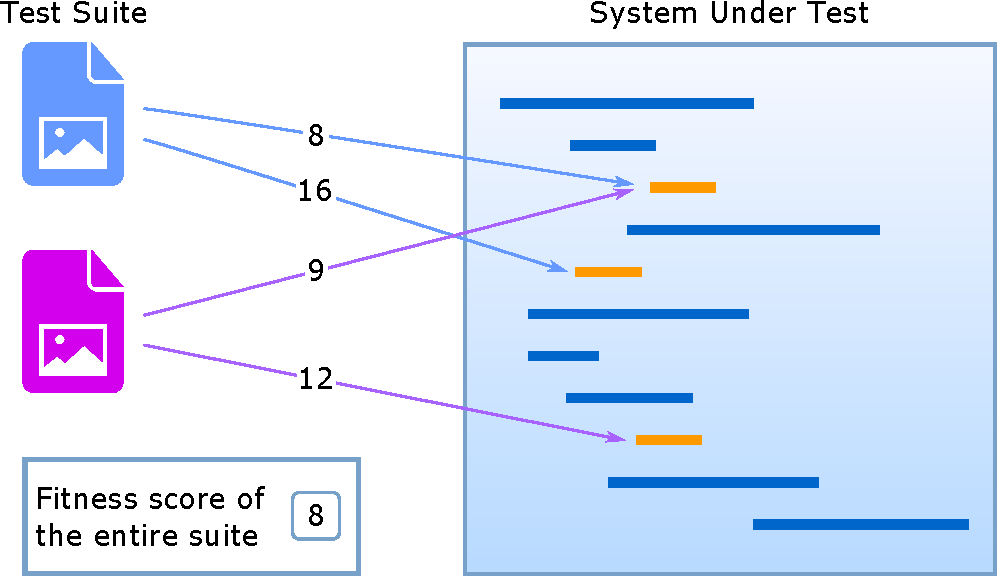
\includegraphics[width=\linewidth]{./div0.pdf}
  \caption{Division By Zero Fitness Score Calculation. Orange blocks indicate division instructions, while
  the numbers on the arrows represent divisors achieved by an input file. The fitness score for the entire
  suite is the minimal attained divisor.}
  \label{fig:div0}
\end{figure}

However, this assignment on its own is not very beneficial
to the diversity of the inputs' gene pool as it makes it converge to smaller files with a minimum
number of executed divisions as long as there is at least one divisor close to zero. Such a constriction opposes the
goal of triggering a division exception as it artificially and unnecessarily limits the number of sites
that are considered for exploration. 

To counteract this effect additional secondary objectives were put in place. The first secondary objective is
the \texttt{MaximizeDivisionsSecondaryObjective} whose goal is to enlarge the number of sites in the
program under test that are being explored by the search process. This is achieved by increasing the number of
division instructions covered by a suite. Using only this single secondary objective, however, causes 
individuals to simply grow in size over the course of evolution, while keeping at least one close-to-zero
divisor. While this is beneficial to the diversity of the suites, it imposes an unwelcome strain on the
performance, which is why another secondary -- or rather a tertiary -- objective has been added: the
\texttt{MinimizeCumulativeZeroDistanceSecondaryObjective}. The goal of this objective is to prevent an
uncontrolled growth and ensure overall improvement of quality of the individuals by keeping the cumulative
divisor distance to zero as small as possible.

The pintool component of the \texttt{Division by Zero} fitness function intercepts all invocations
of the \texttt{DIV} and \texttt{IDIV} x86 instructions at runtime and records the divisor value in a list,
which is associated with the address of the instruction in question by means of a map container. When the
execution of the system under test has ended, for each division instruction the pintool keeps only the divisor
with the smallest zero distance when packing the message to be sent out to its \java fitness function
counterpart.
There is a reason behind selecting the best divisor only after the main runtime instead of doing it on-the-fly,
even though it wastes some memory space for storing all observed divisors. This is an instance of the classical
runtime vs memory requirement trade-off: by having injected code simply append any new value to a list
instead of doing comparisons to decide whether to keep or reject the new value, the code is simple enough to
be inlined and thus performs considerably faster; and with main memory being available in abundance on  modern
computers and execution speed being the most limiting factor, it seems like a reasonable trade-off to make.

Because the \texttt{Division by Zero} fitness function is meant to be used for vulnerability scanning, it is
exclusively compatible with the singleton population evolution mode introduced in \cref{sec:memcov}. The \java
component of this fitness function keeps a record of all executed division instructions alongside the absolute
value of their divisor closest to zero for each file in a suite. The overall fitness score of the entire suite
is then determined by finding the minimal divisor distance over all division instructions over all files in
the suite as sketched in \cref{fig:div0}.

As previously suggested, this fitness function currently only supports integer based division instructions
because \pin imposes a limitation on retrieving floating point values from
registers\footnote{\url{https://software.intel.com/sites/landingpage/pintool/docs/67254/Pin/html/index.html\#FP}}.
Working around this and adding support for \texttt{SIMD} instructions are some planned future improvements.

Intuitively, it is unusual for valid, well formed inputs to cause divisions by zero in the program under
test. It is therefore recommended to use the schema violation feature described in \cref{sec:local}, which is
capable of producing values beyond the range of validity, in order to increase the chances of actually
triggering arithmetic exceptions.

%### 
\subsubsection{Integer Overflow Fitness Function}
%### 
Continuing in the vein of fitness functions specialized in narrow categories of vulnerabilities, the next
fitness function is the \texttt{Integer Overflow Fitness Function}. Just as the name suggests, its aim is to
guide the evolution of inputs towards causing an unhandled integer overflow. Integer overflows are often
suitable as vessels for denial of service attacks as well as access control attacks, and therefore of
critical severity. 

In order to achieve its goal, the \texttt{Integer Overflow} fitness function uses its pintool component to
monitor all invocations of \texttt{MUL}, \texttt{IMUL} and \texttt{ADD} x86 instructions in the targeted
program and examine their arguments. Because overflows arise when two large integers are multiplied or added
such that the resulting value no longer fits in the size of an integer, this fitness function quite simply
favors larger arguments for those arithmetic operations. Quite similarly to the \texttt{Division by Zero}
fitness function, for each individual instruction a list of argument pairs is kept, from which the largest pair
is selected when reporting fitness to the \java master process. Once again, this is done for performance
reasons.
 
As this fitness function is also vulnerability-oriented, it is restricted to the singleton population usage
scenario and the fitness score of a suite is defined as the sum of the largest argument pair over all sites
and input files. Additionally, it is tentatively advisable to employ the schema violation mechanism to
encourage values outside their legal domains with the aim of increasing the chance of triggering overflows.

This fitness function employs additional secondary objectives that are analogous to those of the
\texttt{Division by Zero} fitness function in that they also aim to increase the number of distinct
potential exploitation sites. They do so by favoring suites with a larger number of unique instructions, while
limiting the number of files in the suites to within a reasonable magnitude.

%### 
\subsubsection{Buffer Overflow Fitness Function}
%###
Yet another fitness function mainly aimed at its own specific class of vulnerabilities, the \texttt{Buffer
Overflow Fitness Function} seeks to identify potential buffer overflows and underflows, which can be highly
exploitable. This fitness function is very roughly based on the \texttt{Memory Access} fitness function,
however, it is technically more involved. 

The main idea behind aiming towards buffer overflows and underflows is deceptively simple: all one has to do
is monitor allocations, reallocations, and deallocations of buffers, record all memory accesses to them, and
favor those that are either at the beginning or end regions over those near the middle.

Unfortunately, the technical implementation of the prototypical pintool for use on Linux operating systems
turns out to be not as straightforward as the idea itself because, for the first time, an instrumentation on
function level is required. This is different from instrumenting applications on the level of individual
instructions or loading and unloading of binary images mainly because there exists a distinct possibility of
interleaved execution in multi-threaded applications. At least the technique for monitoring memory accesses
can be inherited from the \texttt{Memory Access} fitness function, therefore the focus of the problem at hand
rests with the potentially interleaved execution of \texttt{malloc}, \texttt{calloc} and \texttt{realloc} functions,
which are responsible for allocating buffers. 

Before considering concrete solutions, a data model for containing all relevant information must be designed.
For currently allocated buffers a set of \texttt{(rip, start, size)} triples will be kept, where \texttt{start}
and \texttt{size} are the beginning address and the size of the buffer, respectively, and \texttt{rip} is the
address of the instruction executed immediately after the return from the buffer allocating function. It is
used to provide both a distinction between different allocation sites, as well as a grouping criterion for
buffers that serve the same purpose at different times (think of buffer allocations in a loop for processing
subsequent chunks of an input). Logging of \texttt{rip}s arose from the need to uniquely identify different
allocation calls; unfortunately, \pin offers no easy possibility to identify the call site, but it provides
access to the \texttt{rip} out of the box. To ensure that only the currently allocated buffers are stored, an
allocation is removed from the set of recorded allocations whenever a buffer is freed by a call to
\texttt{free}.

This set is just an auxiliary data structure that does not provide any useful information in terms of the
planned fitness score. Therefore, a second data structure is necessary to capture the actual memory accesses
-- an associative mapping from \texttt{rip}s to the maximum access distance from the center of a buffer
pertaining to an allocation before the \texttt{rip}. By using the distance from the center as a metric it
is possible to aim for accesses at both extremes of a buffer, thus giving equal preference to both overflows
and underflows at the same time. More specifically, the \texttt{access distance} of an access at address
\texttt{addr} to a buffer corresponding to the triple \texttt{(rip, start, size)} is calculated as $dist =
|start + \lfloor\frac{size}{2}\rfloor - addr|$. For an example consider \cref{fig:memaccess}: there is a buffer
corresponding to the triple \texttt{(any\_rip, 22, 27)} and two accesses \texttt{x} and \texttt{y} at
addresses 24 and 42 respectively. The center of this buffer is at address $22 + \lfloor\frac{27}{2}\rfloor =
35$. Thus, the access distance of \texttt{x} is $|35 - 24| = 11$ and that of \texttt{y} is $|35 - 42| = 7$.

\begin{figure}[H]
\centering
	\vspace{.5cm}
	\begin{bytefield}{32}
		\bitbox[]{6}{} & 
		\bitlabel{1}{\texttt{start}} &
		\bitbox[]{1}{} &  
		\bitlabel{1}{\texttt{x (dist = 11)}} &
		\bitbox[]{10}{} &  
		\bitlabel{1}{\texttt{center}} &
		\bitbox[]{6}{} &  
		\bitlabel{1}{\texttt{y (dist = 7)}} & 
		\bitbox[]{6}{} &  
		\bitlabel{1}{\texttt{start + size}} \\
		\bitheader[lsb=16]{22,24,35,42,49} \\
		\bitbox[tbr]{6}{\tiny ambient \\ \tiny variables} &
		\bitbox[tb]{2}{} &
		\bitbox[tb]{1}{\color{lightgray}\rule{\width}{\height}} &
		\bitbox[bt]{17}{\ \ \ \ \ \ \ \ \ \ \ \ \ \ \ \ \ \ buffer} &
		\bitbox[tb]{1}{\color{lightgray}\rule{\width}{\height}} &
		\bitbox[tbr]{6}{} &
		\bitbox[tbl]{6}{\tiny ambient \\ \tiny variables}
	\end{bytefield}
	\caption{Memory Access Distance}
	\label{fig:memaccess}
\end{figure}

Having established the desired data model and coming back to the problem of capturing buffer allocations as they
happen in a possibly multi-threaded application, a solution is to use Pin's API for instrumentation
at procedure level and have two callbacks -- one at the entry of the allocation function, and the other at the
exit. With this setup the \texttt{rip} and the \texttt{size} values are accessible to the first callback and
\texttt{rip} and \texttt{start} to the second. So the idea is to reserve a triple \texttt{(rip, unknown, size)}
in the first callback, and later find it and fill in the \texttt{start} value in the second. Unfortunately, due
to interleaved execution, it is possible for two threads to enter an allocation function with the same
\texttt{rip} at the same time, so that when one of them returns activating the second callback, it has no way
of assigning the \texttt{start} value to the correct reserved entry. The obvious way to fix this is to
additionally keep the \texttt{thread\_id}, which, luckily, \pin also provides. This would somewhat bloat the
auxiliary data structure to a set of \texttt{(thread\_id, rip, start, size)} with probably very little
variation in the first value, so it seems like a waste of space. An optimization can be achieved by using
thread local storage facilities provided by \pin and reserve preliminary triples there, which requires
additional synchronization when moving the completed triples into the common auxiliary data structure. This
solution would be perfectly acceptable, if it weren't for a small comment in the examples section of Pin's
documentation\footnote{\url{https://software.intel.com/sites/landingpage/pintool/docs/67254/Pin/html/\#Invocation}}:
\begin{quote}
{\small IPOINT\_AFTER} is implemented by instrumenting each return instruction in a routine. \pin tries to find
all return instructions, but success is not guaranteed.
\end{quote}
Unfortunately, {\small IPOINT\_AFTER} is exactly the instrumentation point needed to implement the second
callback, which makes the entire contraption unreliable at best and factually wrong at worst.

Luckily, a better solution presented itself: it is possible to replace the allocating functions with variants
that additionally perform the record keeping task.
This is actually exactly what is already used for communicating between the test drivers and their pintools, as
mentioned in \cref{sec:components}, when the pintool replaces the well known functions in the test driver with
its own versions. In this case, however, an additional feature of procedure replacement was used: the signature
change. This is best explained using a simple example of the \texttt{malloc} function.

The original version has the signature \mintinline{cpp}{void *malloc(size_t size)}. In order to be able to
record the \texttt{rip} of an invocation, the malloc wrapper function has to have a signature of 
\mintinline{cpp}{void *mallocWrapper(size_t size, void *rip)}, whereby \pin would fill in the second argument
at the moment of invocation. The code of this wrapper function is roughly sketched in \cref{lst:mallocwrapper}.

\begin{listing}[htb]
\centering
\begin{cppcode}
void *MallocWrapper(size_t size, void *rip) {
	void *start = malloc(size); // call original malloc
	allocations.insert(Allocation_T(rip, start, size)); // store triple
	return start; // return original value
}
\end{cppcode}
\caption{MallocWrapper Code Sketch}
\label{lst:mallocwrapper}
\end{listing}

The wrapper function first invokes the original \texttt{malloc} and stores its return value. At this point the
wrapper has access to all three necessary values at once and stores the triple \texttt{(rip, start, size)}
before returning the original return value. Please regard the code presented in \cref{lst:mallocwrapper} as
pseudocode because the actual code is somewhat more involved.

Firstly, calling the original \texttt{malloc} function is not as straightforward because \pin has its own
implementation of \texttt{malloc} that uses its own allocator and thus is not compatible with the intended
\texttt{malloc} call as any attempt to free the returned buffer from inside the instrumented program using a
call to its \texttt{free} function will result in a segmentation error. Additionally, the space reserved for
\pin allocations is rather limited, which also makes it infeasible to patch the \texttt{free} calls
accordingly. Even if \pin did not override \texttt{malloc}, simply inserting a call to it would result in an
infinite loop as \pin would try to replace this call by the wrapper as well. Therefore the invocation is
actually a call to a special method in Pin's API that allows execution of the original function
without it being instrumented.

Secondly, additional checks are performed inside the wrapper, such as ensuring that only calls pertaining to
the targeted binary image are recorded or testing the return value for being \texttt{NULL} and treating this
case specially.

The allocation functions \texttt{calloc} and \texttt{realloc} are treated analogously to \texttt{malloc}, but
\texttt{free} is actually not replaced at all because it is sufficient to add a callback at its entry site
(which, luckily, \pin guarantees to work) that will simply remove a triple with the \texttt{start} value equal
to the argument of \texttt{free} if one is found.

As mentioned previously, the fitness information, that the pintool of the \texttt{Buffer Overflow
Fitness Function} sends to its \java counterpart, is the memory access map, which, in contrast to the
\texttt{Division by Zero} and \texttt{Integer Overflow} fitness functions is updated in-place and not only
after the processing of an input file. Because memory accesses are much more numerous than e.g.\ \texttt{DIV}
or \texttt{MUL} instruction invocations, the reasonable choice in the memory-speed trade-off is somewhat offset.

The \java part of this fitness function aims to maximize the distance of the accesses from their
respective buffer's centers, and by employing additional secondary objectives, it also aims to enlarge the
number of accessed buffers as well as the cumulative access distance in a suite, while preventing the suites
from bloating by favoring smaller ones if all their previously mentioned characteristics are equal.

As is the case with several previous fitness functions, this fitness function is also geared toward finding
vulnerabilities and therefore employs the singleton population paradigm.
The fitness score of a suite is calculated as the maximal access distance over all buffers and input files. 
Also note that it would be infeasible
to count memory accesses outside allocated buffer ranges as out-of-bounds accesses to the buffers themselves because they may well be
just accesses to ambient variables. Therefore this fitness function assigns maximum values to accesses just at
the legal bounds of the buffers and relies on mutations to make it possible to break out of this restriction
and possibly trigger a sought-after vulnerability.
